%% uctest.tex 11/3/94
%% Copyright (C) 1988-2004 Daniel Gildea, BBF, Ethan Munson.
%
% This work may be distributed and/or modified under the
% conditions of the LaTeX Project Public License, either version 1.3
% of this license or (at your option) any later version.
% The latest version of this license is in
%   http://www.latex-project.org/lppl.txt
% and version 1.3 or later is part of all distributions of LaTeX
% version 2003/12/01 or later.
%
% This work has the LPPL maintenance status "maintained".
% 
% The Current Maintainer of this work is Daniel Gildea.

\documentclass[11pt]{ucthesis}
\usepackage[pdftex]{graphicx}

\usepackage{subfigure}
\usepackage{url}
\def\dsp{\def\baselinestretch{2.0}\large\normalsize}
\dsp
\begin{document}

% Declarations for Front Matter

\title{Questioning The NS-3 TCP Implementation and Presenting an Alternative Design}
\author{Allison Hume}
\degreeyear{2016}
\degreemonth{June}
\degree{MASTER OF SCIENCE}
\chair{Professor Katia Obraczka}
\committeememberone{Professor Luca de Alfaro}
\committeemembertwo{Professor Carlos Maltzahn}
%\committeememberthree{Professor Ipsum Lorem}
\numberofmembers{3} %% (including chair) possible: 3, 4, 5, 6
\deanlineone{Tyrus Miller}
\deanlinetwo{Vice Provost and Dean of Graduate Studies}
\deanlinethree{}
\field{Computer Science}
\campus{Santa Cruz}

\begin{frontmatter}

\maketitle

\copyrightpage

\tableofcontents
\listoffigures
\listoftables

\begin{abstract}
The existing TCP implementation in the NS-3 network simulator is not sufficiently accurate to be useful for making comparisons between different congestion control algorithms. This work demonstrates how the current implementations in both the production and development versions of the simulator differ from results presented in previous literature. It is observed that errors are introduced by the lack of a consistent, extensible design for congestion control. The main contribution is a design that will make the NS-3 TCP implementation more accurate and make it easier for new congestion control algorithms to be implemented in the simulator.  
\end{abstract}

%\begin{dedication}
%\null\vfil
%{\large
%\begin{center}
%To myself,\\\vspace{12pt}
%Perry H. Disdainful,\\\vspace{12pt}
%the only person worthy of my company.
%\end{center}}
%\vfil\null
%\end{dedication}


\begin{acknowledgements}

My deepest gratitude goes to my parents. Thank you for giving me an education, not just sending me to school. Thank you for teaching me to love books, to be persistent, and to question ideas. Thank you Dad for a childhood full of random explanations that made me interested in the world around me. Thank you Mom for encouraging me to ask for help. Thank you both for providing everything I have needed and so much more. And of course, Lydia, thank you for not always letting me read, but for sometimes making play. I am incredibly fortunate to have the family that I do and I thank you all for loving me unconditionally and letting me always be myself.

Thank you Jacopo, for being able to play so many roles in my life. Thank you for being part of a crucial step in my educational path, and for helping me through all my road-blocks, real or imagined. ``Being there" has taken many forms but there you have been throughout this process and for that I am very grateful.

Lastly, where would I be without my friends? Dora and Diana, thank you for your readiness to ``do non-stressful things for the purpose of relaxation," and for being happy to talk about anything but our theses. And, of course, thank you TFC. Food=Love.

\end{acknowledgements}

\end{frontmatter}

%\part{First Part}

\chapter{Introduction}

\section{Motivation}
Simulators are a very important tool for the networking community. In contrast to live hardware, simulators allow experiments to cover a large number of topologies and allow researchers to experiment easily with changes in experiment or protocol settings. One critical feature that a network simulator must offer is the ability to run code that is as close to live as possible. Code should reflect the state of the art in hardware and be easily modified and expanded so that researchers who want to experiment with new protocols can easily add them to the existing set of code. 

One active area of research in the TCP community is introducing and comparing different congestion control algorithms. Network simulators are essential tools for validating, understanding, and comparing these algorithms and NS-3 and its previous incarnation, NS-2, have a long track record of usage in the TCP community for this purpose \cite{NS2Val}, \cite{NS2WP}. As the simulator has changed and evolved, however, there has not been enough of an effort to continue to validate and understand the simulator itself. The work presented in this paper began as an effort to understand a newly proposed TCP congestion control algorithm, TCP Inigo \cite{Inigo}, using NS-3 as a simulator platform. It became clear, however, that the existing TCP implementation in NS-3, while potentially sufficient for comparing aggregate metrics such as throughput, or for supporting higher level protocols, may not be robust enough to support the detailed analysis that is necessary to understand and compare congestion control algorithms.

Figure \ref{WNS3} shows a trace of the congestion window for TCP Westwood using an experiment first mentioned in Gangadhar et al\cite{NS3W}. The plot on the left shows the experiment run on NS-3 version 3.24 while the plot on the right shows the same experiment run on NS-3 version 3.25.  This figure shows that the implementation of TCP Westwood has changed drastically between the two implementations. How can researchers trust simulators to compare different versions of TCP when established protocols are not consistent between simulator versions? This work has been motivated by these findings, and by the difficulties encountered in adding a new congestion control algorithm to NS-3. The main contribution in this work is a design for simulated TCP that will be easier to maintain, and more extensible, than existing designs. The design will be presented after a brief background on TCP congestion control and existing TCP code designs. This work also presents results that question the existing TCP implementation in NS-3, lending weight to the argument that a comprehensive design evaluation, as well as formal validation process, is very much needed. 

\begin{figure}[!t]
\centering
%\subfigure{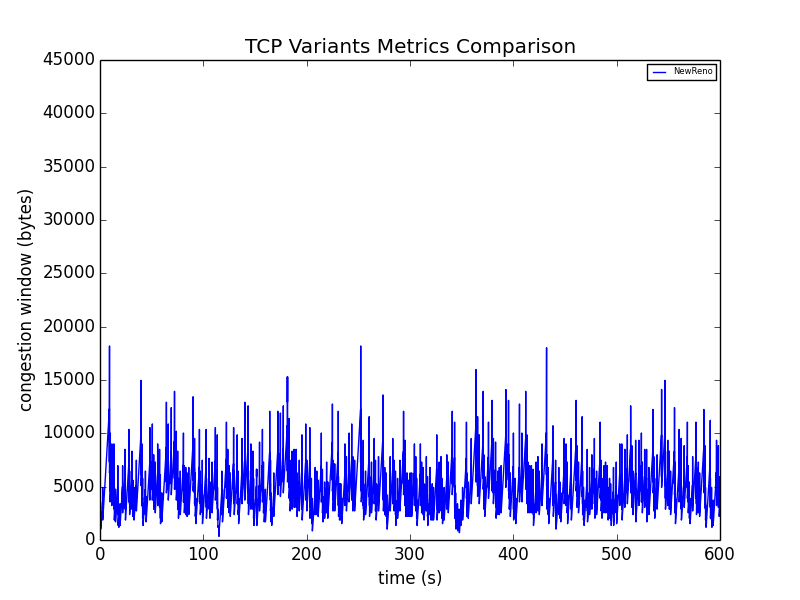
\includegraphics[trim=1cm 6.5cm 2.2cm 7.6cm, clip=true, scale=0.23]{inigo_test_results/repeatWestwoodPaper/WNS3NR.pdf}\label{a}}
%\subfigure{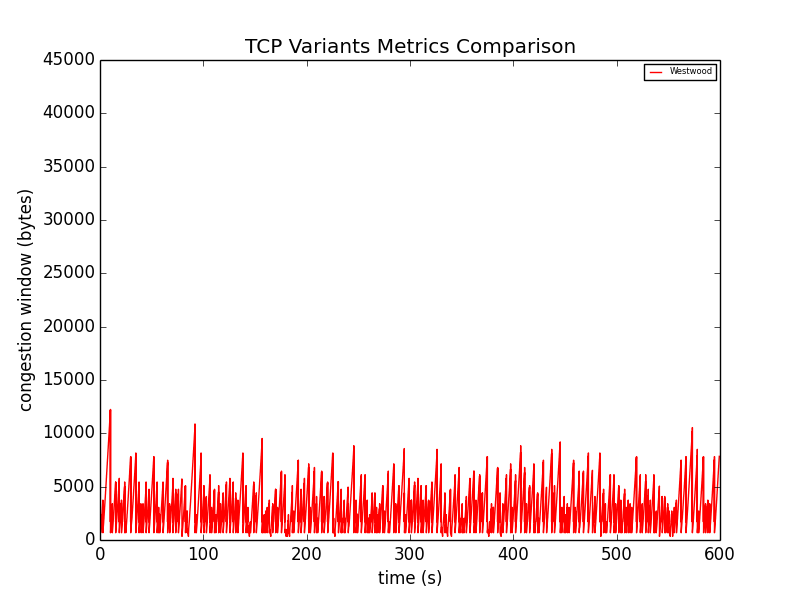
\includegraphics[trim=1cm 6.5cm 2.2cm 7.6cm, clip=true, scale=0.23]{inigo_test_results/repeatWestwoodPaper/WNS3W.pdf}\label{b}}
%\subfigure{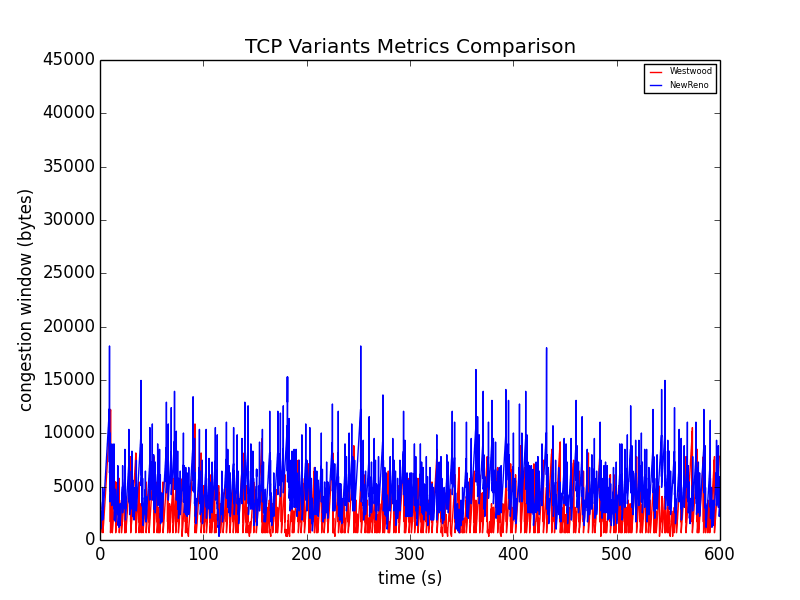
\includegraphics[trim=1cm 6.5cm 2.2cm 7.2cm, clip=true, scale=0.2]{inigo_test_results/repeatWestwoodPaper/WNS3Both.pdf}\label{a}}
%\subfigure{\includegraphics[trim=1cm 6.5cm 2.2cm 7.6cm, clip=true, scale=0.23]{inigo_test_results/repeatWestwoodPaper/NS3PROD/output/WNS3ProdNR.pdf}\label{c}}
\subfigure{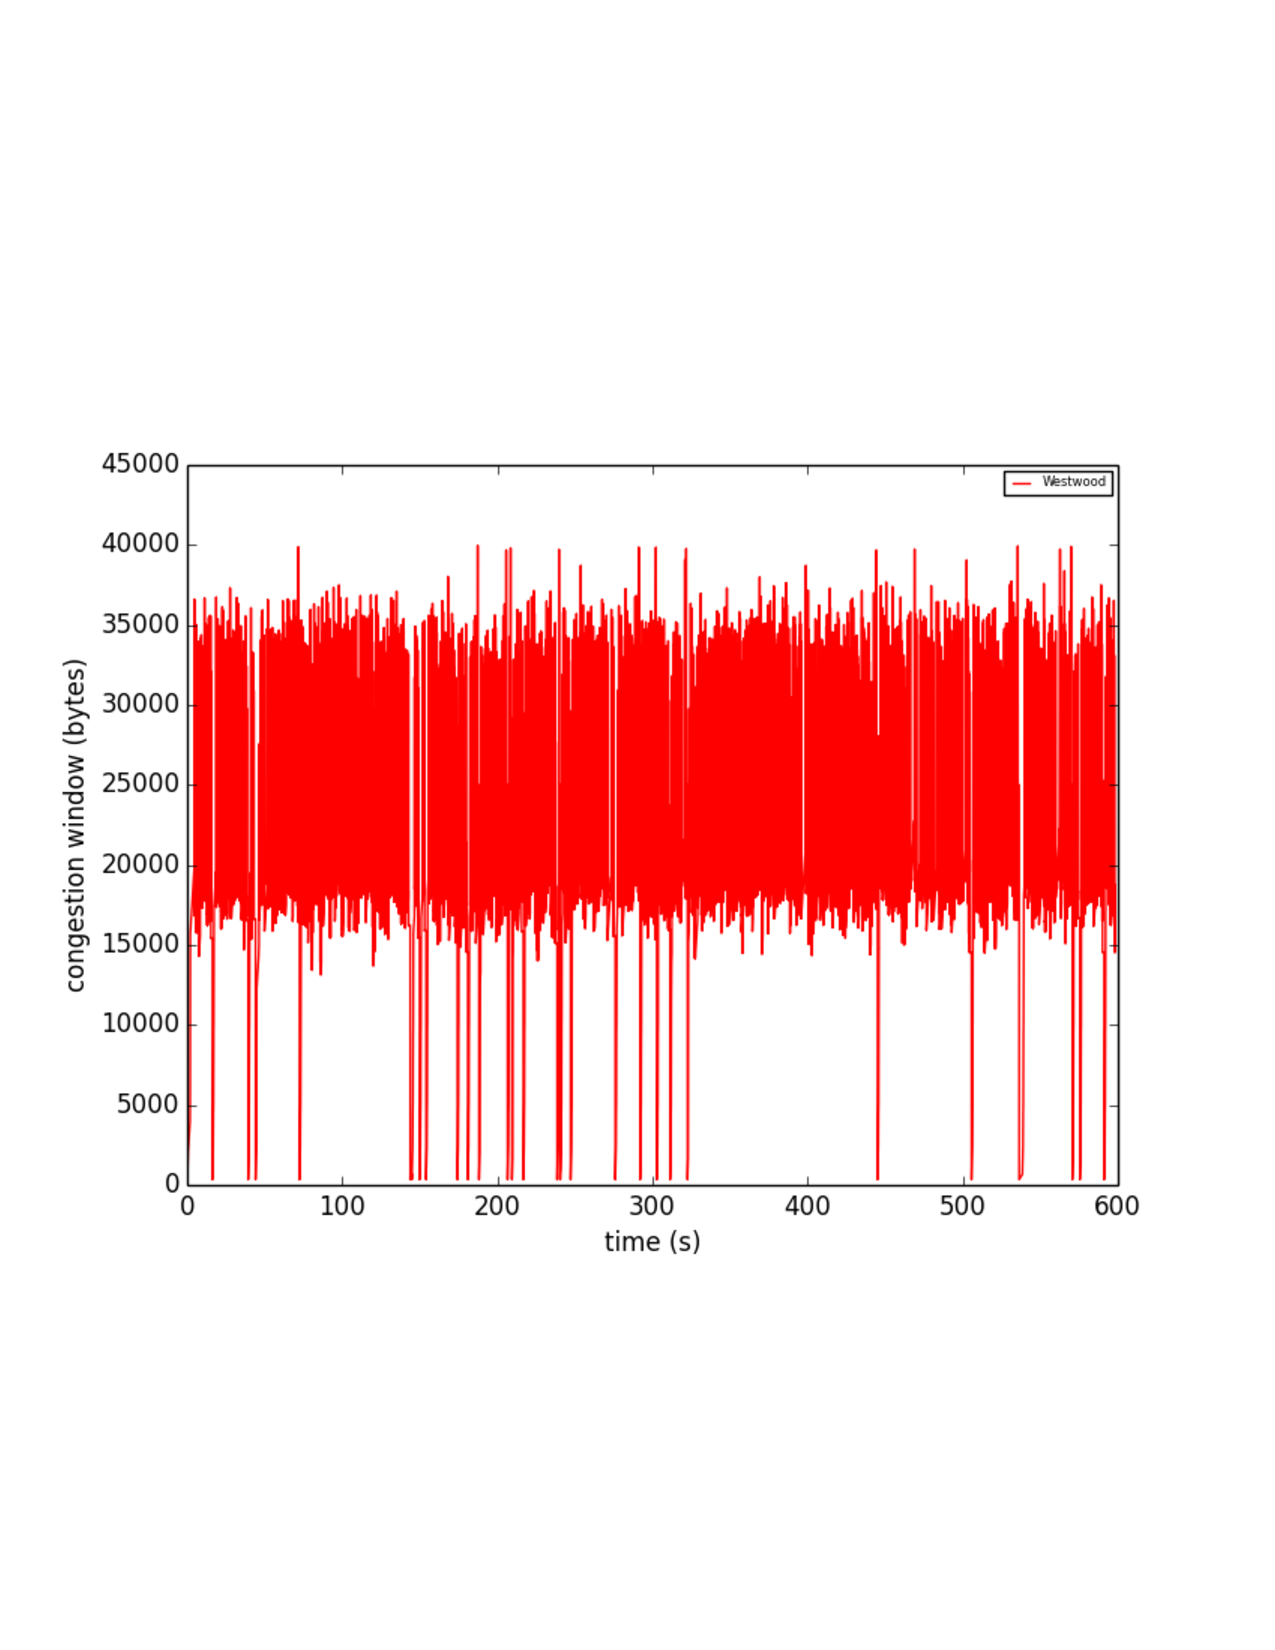
\includegraphics[trim=1cm 6.5cm 2.2cm 7.6cm, clip=true, scale=0.23]{inigo_test_results/repeatWestwoodPaper/NS3PROD/output/WNS3ProdW.pdf}\label{d}}
%\subfigure{\includegraphics[trim=1cm 6.5cm 2.2cm 7.6cm, clip=true, scale=0.25]{inigo_test_results/repeatWestwoodPaper/NS3PROD/output/WNS3ProdAll.pdf}\label{e}}
%\subfigure{\includegraphics[trim=1cm 6.5cm 2.2cm 7.6cm, clip=true, scale=0.23]{inigo_test_results/repeatWestwoodPaper/finalRound/POST25/NewRenoP25.pdf}\label{f}}
\subfigure{\includegraphics[trim=1cm 6.5cm 2.2cm 7.6cm, clip=true, scale=0.23]{inigo_test_results/repeatWestwoodPaper/finalRound/POST25/WestwoodP25.pdf}\label{g}}
%\subfigure{\includegraphics[trim=1cm 6.5cm 2.2cm 7.6cm, clip=true, scale=0.25]{inigo_test_results/repeatWestwoodPaper/finalRound/POST25/WestwoodPlusP25.pdf}\label{h}}
\caption{A 600 second trace of the congestion window of TCP Westwood. Experiment from Gangadhar et al\cite{NS3W} run on both NS-3 version 3.24 and 3.25. }
\label{WNS3}
\end{figure}

\section{Background}

Congestion control in TCP involves the interaction of two main variables: congestion window (cwnd) and slow start threshold (ssth). The TCP sender uses cwnd to adjust its rate of transmission and ssth is used to choose the algorithm by which cwnd is computed. Originally, congestion control was defined by four algorithms: slow start, congestion avoidance, fast retransmit, and fast recovery \cite{RFC5681}. Slow start and congestion avoidance are the two algorithms used by the sender to compute cwnd: slow start is used if cwnd is below ssthresh, and congestion avoidance otherwise. The slow start algorithm is used at the beginning of transmission, or after a congestion event causes cwnd to fall below ssth, and increments cwnd exponentially until a congestion event occurs or ssthresh is reached. The congestion avoidance algorithm increments cwnd more slowly, until a congestion event occurs. The fast retransmit algorithm is used to detect and repair loss based on incoming duplicate ACKs and the fast recovery algorithm is used to adjust cwnd until a non-duplicate ACK arrives. 

Congestion control algorithms refer to specific implementations of those four algorithms, and potentially additional components such as Selective Acknowledgements (SACK), which make it possible for the receiver to acknowledge scattered blocks of data, not just a continuous block. Not all algorithms, however, may differ between different congestion control algorithms. For example, the TCP Westwood \cite{WW} congestion control algorithm is a modification of the TCP Reno congestion control algorithm that changes only how cwnd and ssth are changed after three duplicate ACKs or a timeout. While Reno halves the congestion window after three duplicate ACKs, Westwood uses a bandwidth estimator to try to match the variables to the currently available bandwidth. The two congestion control algorithms, however, have the same implementation of slow start. 

The previous discussion helps to illuminate some of the challenges that arrise when attempting to implement TCP congestion control in a way that is both efficient and extensible. Extensibility is much more important in a simulator than in hardware. While a new version of TCP congestion control will only be added to the Linux kernel, for example, rarely, new versions will be added to simulators frequently for validation and testing. If the TCP implementation in Linux, therefore, promotes efficiency over extensibility, that is ok. In a simulator, however, lack of extensibility goes directly against the goals of the software. The next section will discuss the recent history of design choices in NS-3 , before a modified design for any simulator is presented. 

\section{Design}

The previous NS3 release, NS-3 version 3.24 has a module called tcp-socket-base that contains the main function from which congestion control functionality is used: ReceivedAck. In that release the functionality in ReceiveAck is minimal, it servers mostly to call the NewAck and DupAck functions, which are defined for each TCP version, in its respective module. In other words, there is one main module for each TCP version containing all code that is required for that specific congestion control algorithm~\cite{NS324Code}. A visual of this design can be seen in the top left of Figure~\ref{fig:design}. The downside of this design approach is code duplication and the difficulty of adding a new congestion control algorithm, although this approach does make the implementation of specific algorithms very clear. 

A recent effort has been underway to refactor the TCP implementation of NS-3 so that the majority of TCP code is shared and only specific congestion control functions must be implemented to define a new version of congestion control~\cite{NS3Patch}. The result of this effort is the recently released NS-3 version 3.25~\cite{NS325Code}. In this version, the ReceivedAck function in tcp-socket-base contains much more functionality and calls more specific, well defined congestion control functions PktsAcked, GetSsThresh, and IncreaseWindow, which are defined in a congestion-ops module as the base class for an congestion control implementation. The top right portion of Figure~\ref{fig:design} summarizes this design. This is a much more extensible approach than the previous design, although great care must be taken to be sure that all shared code is truly generic. As will be discussed further in the results section, that is not currently the case. Another criticism of this design is that currently the functions for TCP NewReno are also implemented in congestion-control-ops, while the functions for TCP Westwood are placed in a separate module. It is not totally clear why this choice was made, although one guess is that it is because NewReno is the default TCP congestion control algorithm. This design also does not make the inheritance clear. It is not obvious, for example, that the Westwood implementation actually uses the SlowStart function defined for NewReno, since SlowStart is not defined in the base class. We believe that this design is moving in the correct direction, but that additional improvements can be made. 

We propose a new design for the NS-3 TCP module that builds off the current modular approach. Our design is based off the following goals for the design of TCP Congestion Control in any simulator:

\textbf{Extensibility:} The primary goal of a simulator is to allow researchers to test and validate new ideas. For the design to support the TCP community in this way it must be straightforward to add new congestion control implementations to an existing code base.

\textbf{Modularity:} Congestion control is characterized by fact that it is made up of a set of algorithms. As such, a modular design is necessary to allow researchers to experiment with the different pieces that make up a congestion control algorithm, without having to create a completely new implementation for each set of existing components. 

Based on these goals, we believe that an implementation of TCP congestion control on a simulator should be modularly built up out of components in such a way that any component is easily switched out or turned off. This would also allow different versions of congestion control to share implementations for specific algorithms. The functionality of ReceivedAck should be reduced slightly, so it does not include specific Fast Retransmit and Fast Recovery algorithms. The tcp-congestion-ops module will remain the base class for all congestion control implementations, without also containing the implementation of NewReno. In addition, the base class will be expanded to also include SlowStart, FastRetransmit, and FastRecovery algorithms. Each function in the base class will have a corresponding module in which all various implementations for those functions will be placed. Lastly, each specific congestion control algorithm will have a module that defines the selection of sub-algorithms of which it is comprised. The bottom portion of Figure \ref{fig:design} summarizes the proposed design. 

\begin{figure}[h!]
\begin{center}
\subfigure{ 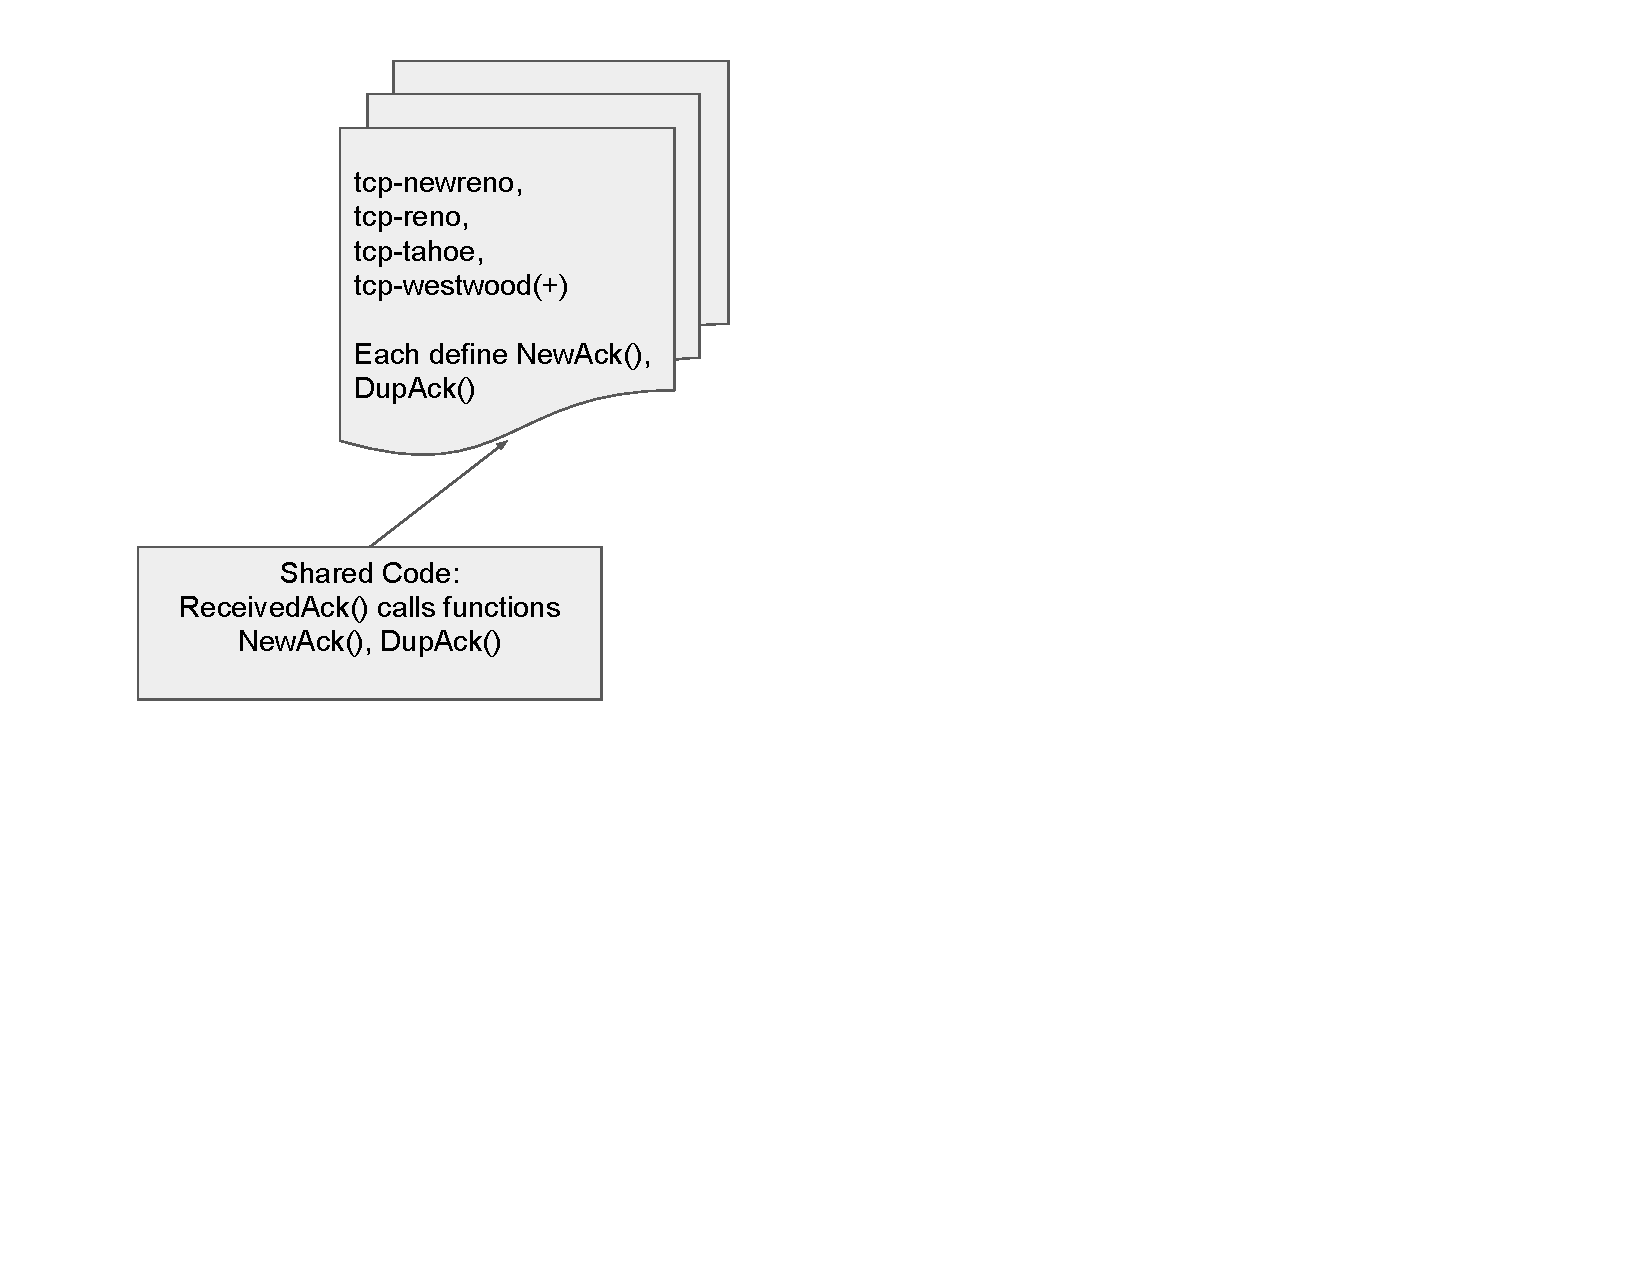
\includegraphics[scale=0.25]{Design1.pdf}\label{a}} 
\subfigure{ 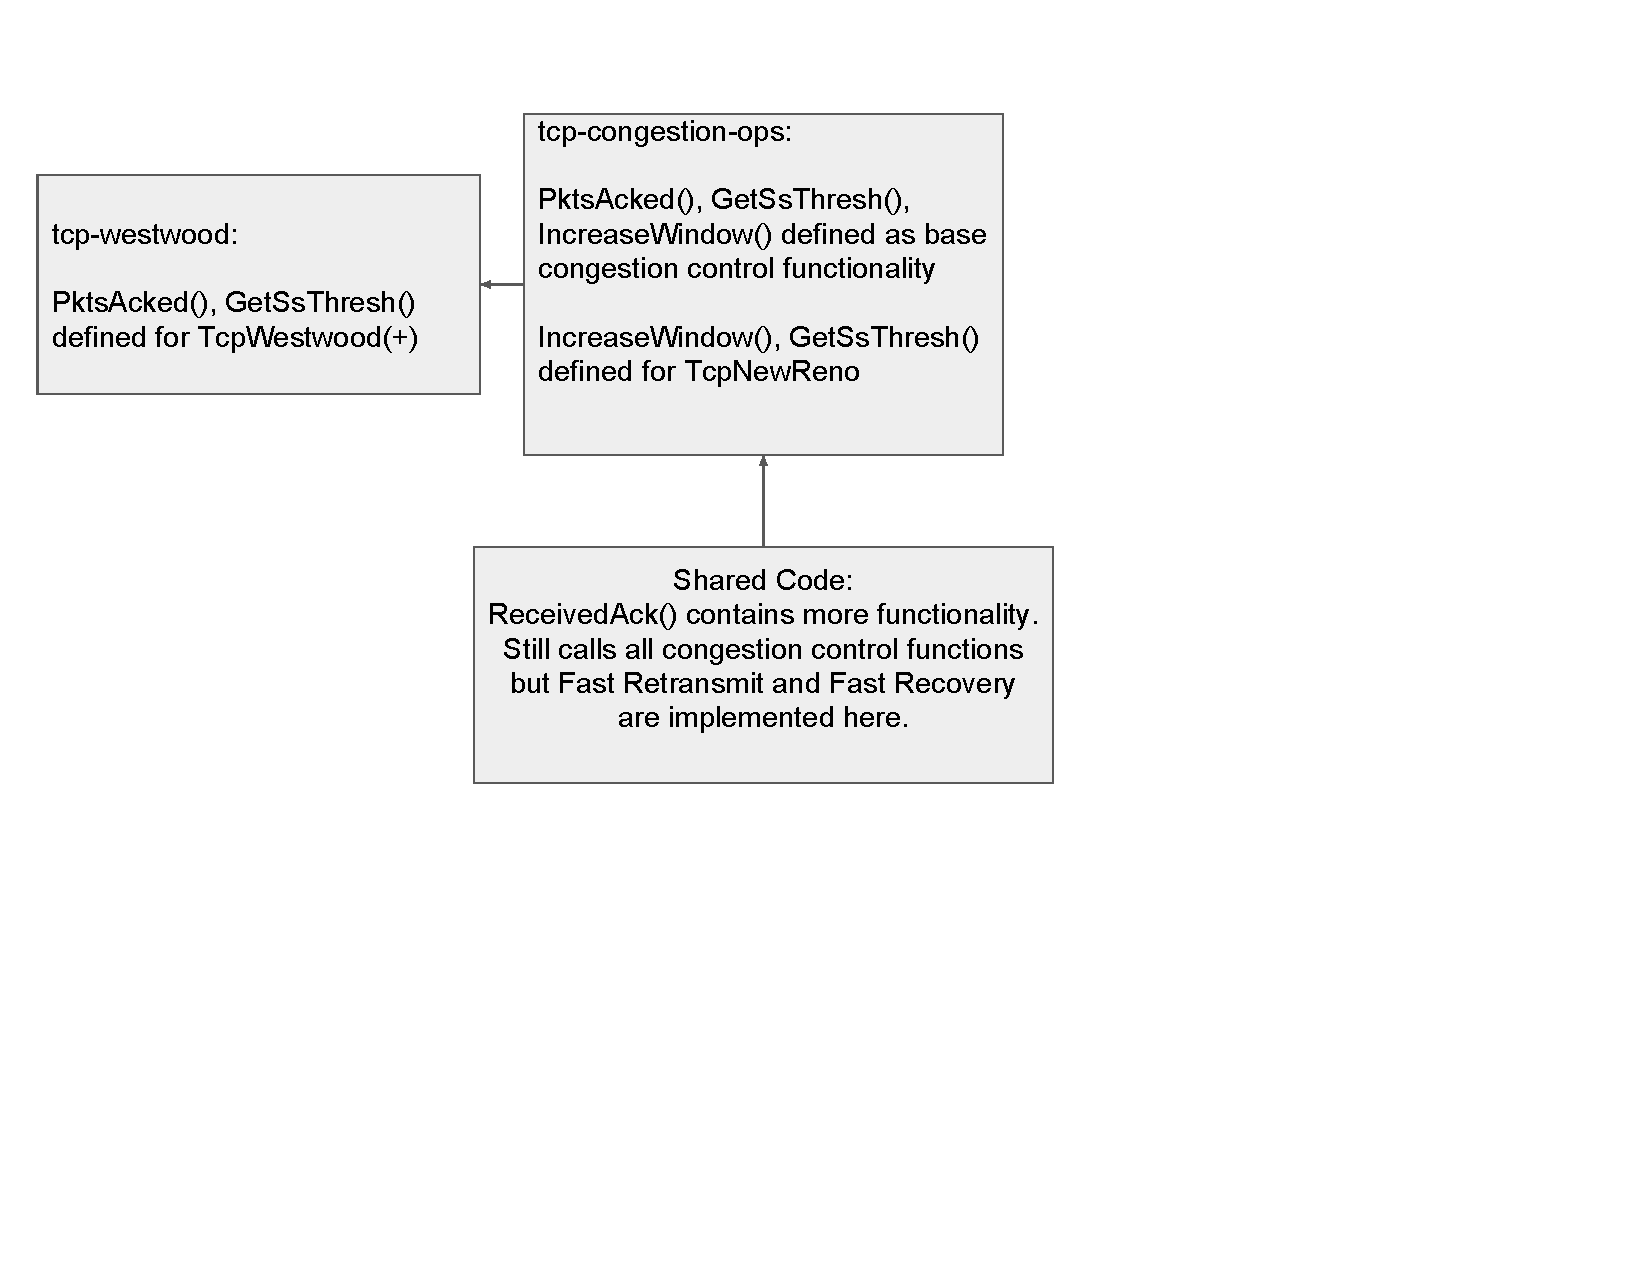
\includegraphics[scale=0.25]{design2.pdf}\label{b}} 
\subfigure{ 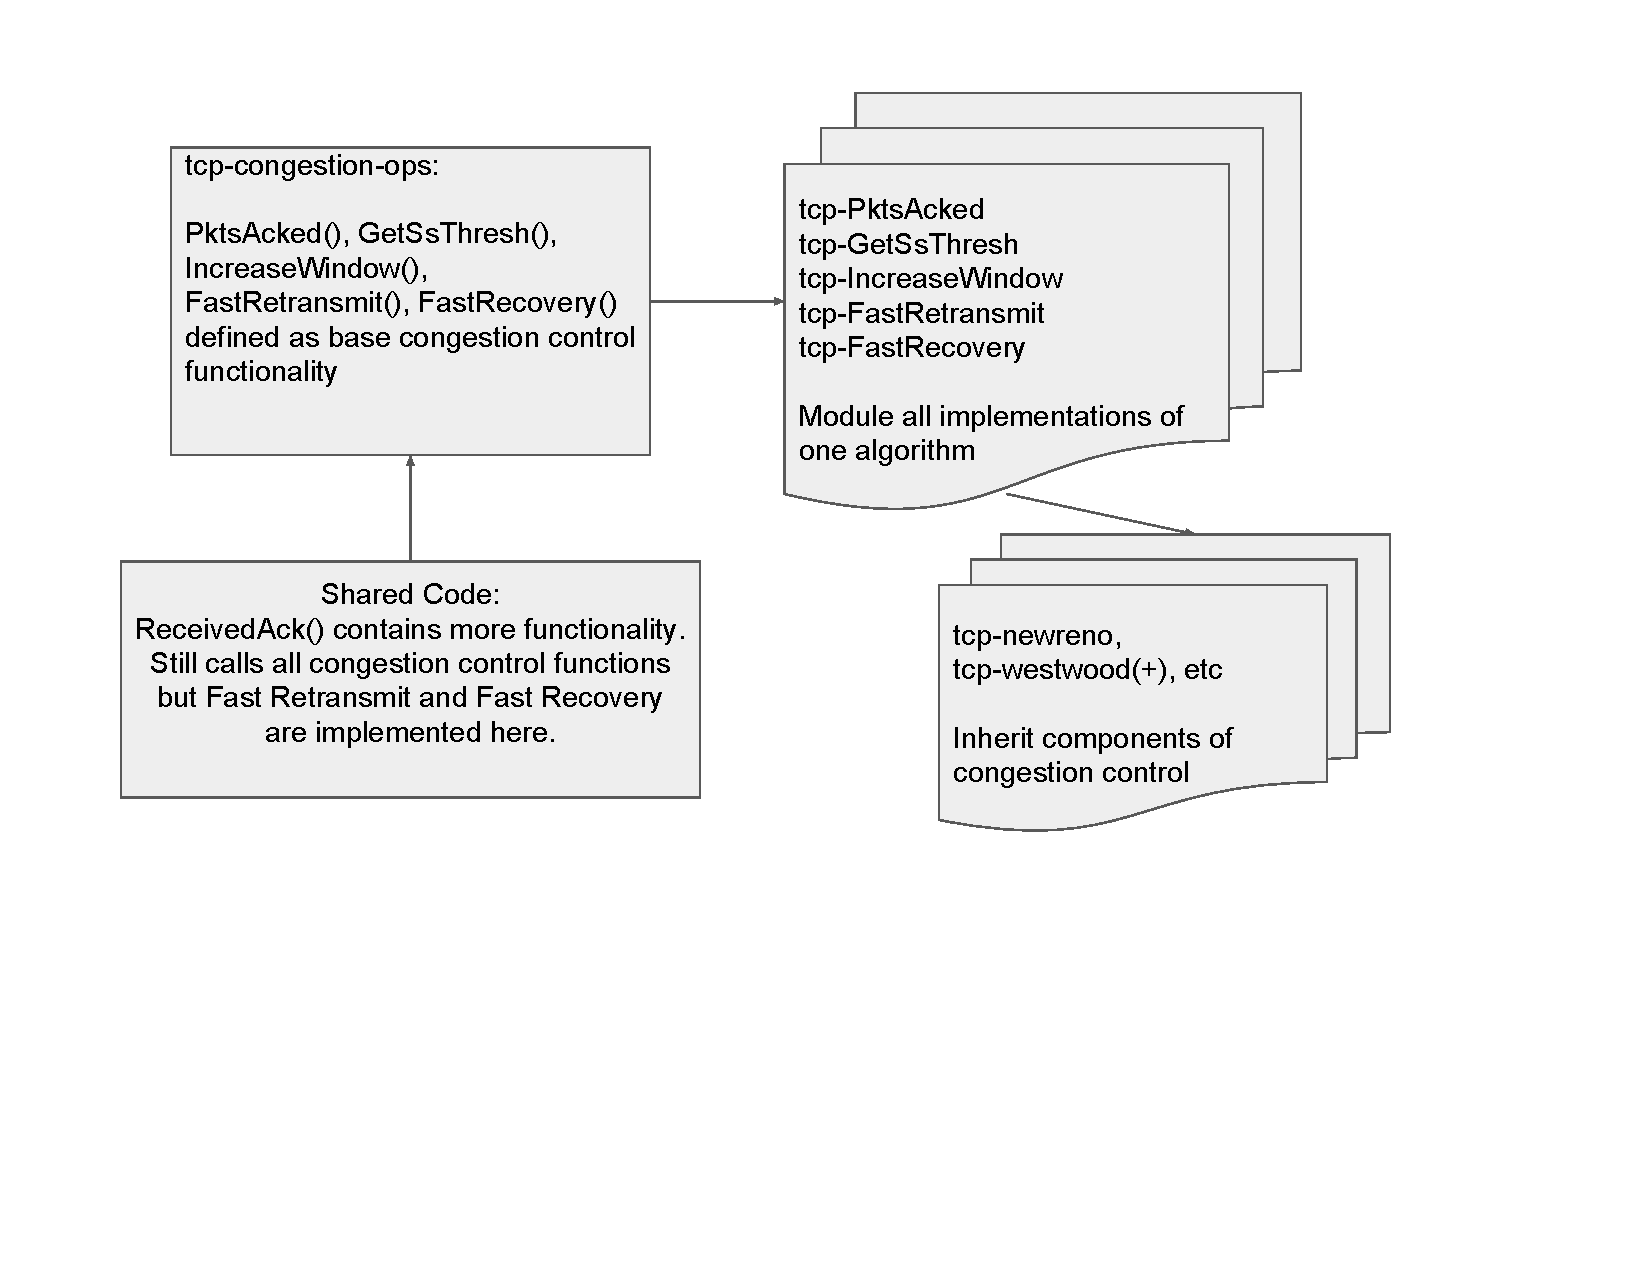
\includegraphics[scale=0.3]{design3.pdf}\label{c}} 
\end{center}
\caption{Diagrams showing the TCP Congestion Control designs for NS3 versions 3.24 and 3.25 (from top left) as well as the design proposed here (bottom).}
\label{fig:design}
\end{figure}

\section{Related Work}

In 2006 there was a significant effort performed by Wei and Cao \cite{NS2Linux} to improve the extensibility, validity, and performance of NS-2 by bringing the TCP implementation closer to the Linux TCP implementation. Not all of their improvements exist currently in NS-3 and this work is very similar in motivation to their work. The main difference is that this work also aims to provide a framework for future congestion control algorithms by promoting a design that allows explicit inheritance of congestion control algorithms, when new algorithms are modifications of previous algorithms. 

In 2015 Casoni et al \cite{NS3Val} performed a validation of NS-3 congestion control algorithms by comparing the operation of those algorithms to the Linux implementations. Since 2015 the NS-3 TCP implementation has been refactored, so their work is an important result for ensuring repeatability. This work attempts to go farther that verification by suggestion design changes to improve the extensibility and accuracy of the NS-3 TCP implementation. 

Bateman and Bhatti \cite{NS2TCPQ} studied the versions of TCP congestion control that existed in the NS-2 simulator in 2010 and found that, using Jain's fairness index as a metric, there were significant variations between the simulator and their physical testbed. This work is an important precedent for questioning the validity of TCP congestion control algorithms in simulators. Instead of using the fairness index as a metric, however, this work investigates congestion window, threshold value, and queue length as comparison metrics in order to make more specific comparisons and as a starting place for identifying what aspects of the implementation cause issues to occur. 

\section{Results} %do generic writeup of experiments also

\begin{table}[!t]
\renewcommand{\arraystretch}{1.3}
\caption{Summary of experiment parameters} 
\label{table:exps}
\centering
\begin{tabular}{|c||c||c||c||c||c|}
\hline
\textbf{Origin} & \textbf{Figure} & \textbf{Bottleneck Link} & \textbf{Access Link} & \textbf{MTU Size} & \textbf{Rate of Packet Loss}\\ 
\hline
Gangadhar et al\cite{NS3W} & Figure \ref{WNS3} & 2 Mbps, 0.01ms delay & 10 Mbps, 45ms delay & 400 B & $5*10^{-3}$\\
(tcp-variants-comparison in NS-3 examples) & Figure \ref{fig:NS2Good} &  &  &  & 0 \\
\hline
Casoni et al\cite{NS3Val} & Figure \ref{fig:NS3Val} & 10 Mbps, 25ms delay & 100Mbps, 1ns delay & 1500 B & $10^{-3}$\\
\hline
Grieco et al\cite{NS2WP} & Figure \ref{fig:NS2Good} & 2Mbps, 125ms delay & 1Gbps, 0.01ms delay & 1500 B & 0 \\
\hline
\end{tabular}
\end{table}

Different experiments show different levels of variation between the current NS3, ns3-3.25 version and previous results obtained from either NS2, previous versions of NS3, or hardware. Figure~\ref{fig:NS3Val} shows an experiment originally presented in Casoni et al\cite{NS3Val}, who presented results comparing TCP NewReno on NS3 version ns3-3.22 to Linux. Their results showed cwnd and ssth from NS3 both very close in scale and pattern to the values obtained from Linux, although cwnd showed major spikes that were attributed to fast retransmit. Figure~\ref{fig:NS3Val}\ref{a} shows the same experiment repeated on NS3 version ns3-3.24, with results very similar to those in the original publication. The source of the spikes, however, discovered to be the increase of cwnd by one segment for every duplicate ACK after the three duplicate ACKs that initiate fast recovery (section 3.2 of RFC 2582\cite{RFC2582}). Figure~\ref{fig:NS3Val}\ref{b} shows the same experiment with that increase removed. This trace now more closely matches the Linux results presented in Casoni et al\cite{NS3Val}.

One thing that is import to note is that this difference was not the result of a bug in NS3. The code very closely follows the RFC, however the Linux TCP implementation handles fast recovery differently. In the Linux implementation cwnd holds the valid number of segments allowed to be outstanding in the network throughout fast recovery, it does not require arbitrary adjusting of the congestion window \cite{NS3Val} \cite{LinuxTCP}. The important point here is that, in order to disable fast recovery, the code for fast recovery had to be tracked down and commented out within the shared code base. The current design of TCP in NS3 allows no option for changing or disabling Fast Retransmit and Fast Recovery algorithms. In different scenarios you may want different implementations one algorithm, or, as in this case, simply to turn it off. Commenting out sections of code is a very error prone method of achieving that result. 

Figure~\ref{fig:NS3Val}\ref{c} and \ref{d} show the same set of experiments, but run on NS3 ns3-3.25 version, with the refactored TCP. It is important to reiterate that, although the intention of this refactoring was to make the TCP congestion control design modular and extensible, it was still necessary to manually find and comment out the relevant lines of code corresponding to fast recovery. Although there is not a drastic difference between the results for the two versions of NS3, the new version does respond differently to the removal of the fast recovery algorithm. %finish this if you find out what causes slow start to start randomly

%\begin{lstlisting}
%if (Dupack) {
%   if (congState == TcpSocketState::CA_RECOVERY) {                                                                                                                          
 %     m_tcb->m_cWnd += m_tcb->m_segmentSize;                                                                                                                                                          
 %        SendPendingData (m_connected); } }
%\end{lstlisting}

\begin{figure}[h!]
\begin{center}
%\subfigure{ \includegraphics[trim=1cm 6.5cm 2.2cm 7.6cm, clip=true, scale=0.23]{inigo_test_results/repeatValidationPaper/finalVersion/Dev.pdf}\label{a}} %dev - with refactor 
%\subfigure{ \includegraphics[trim=1cm 6.5cm 2.2cm 7.6cm, clip=true, scale=0.23]{inigo_test_results/repeatValidationPaper/finalVersion/PotentialBugFix/DevNOFR.pdf}\label{b}} %dev - with refactor
\subfigure{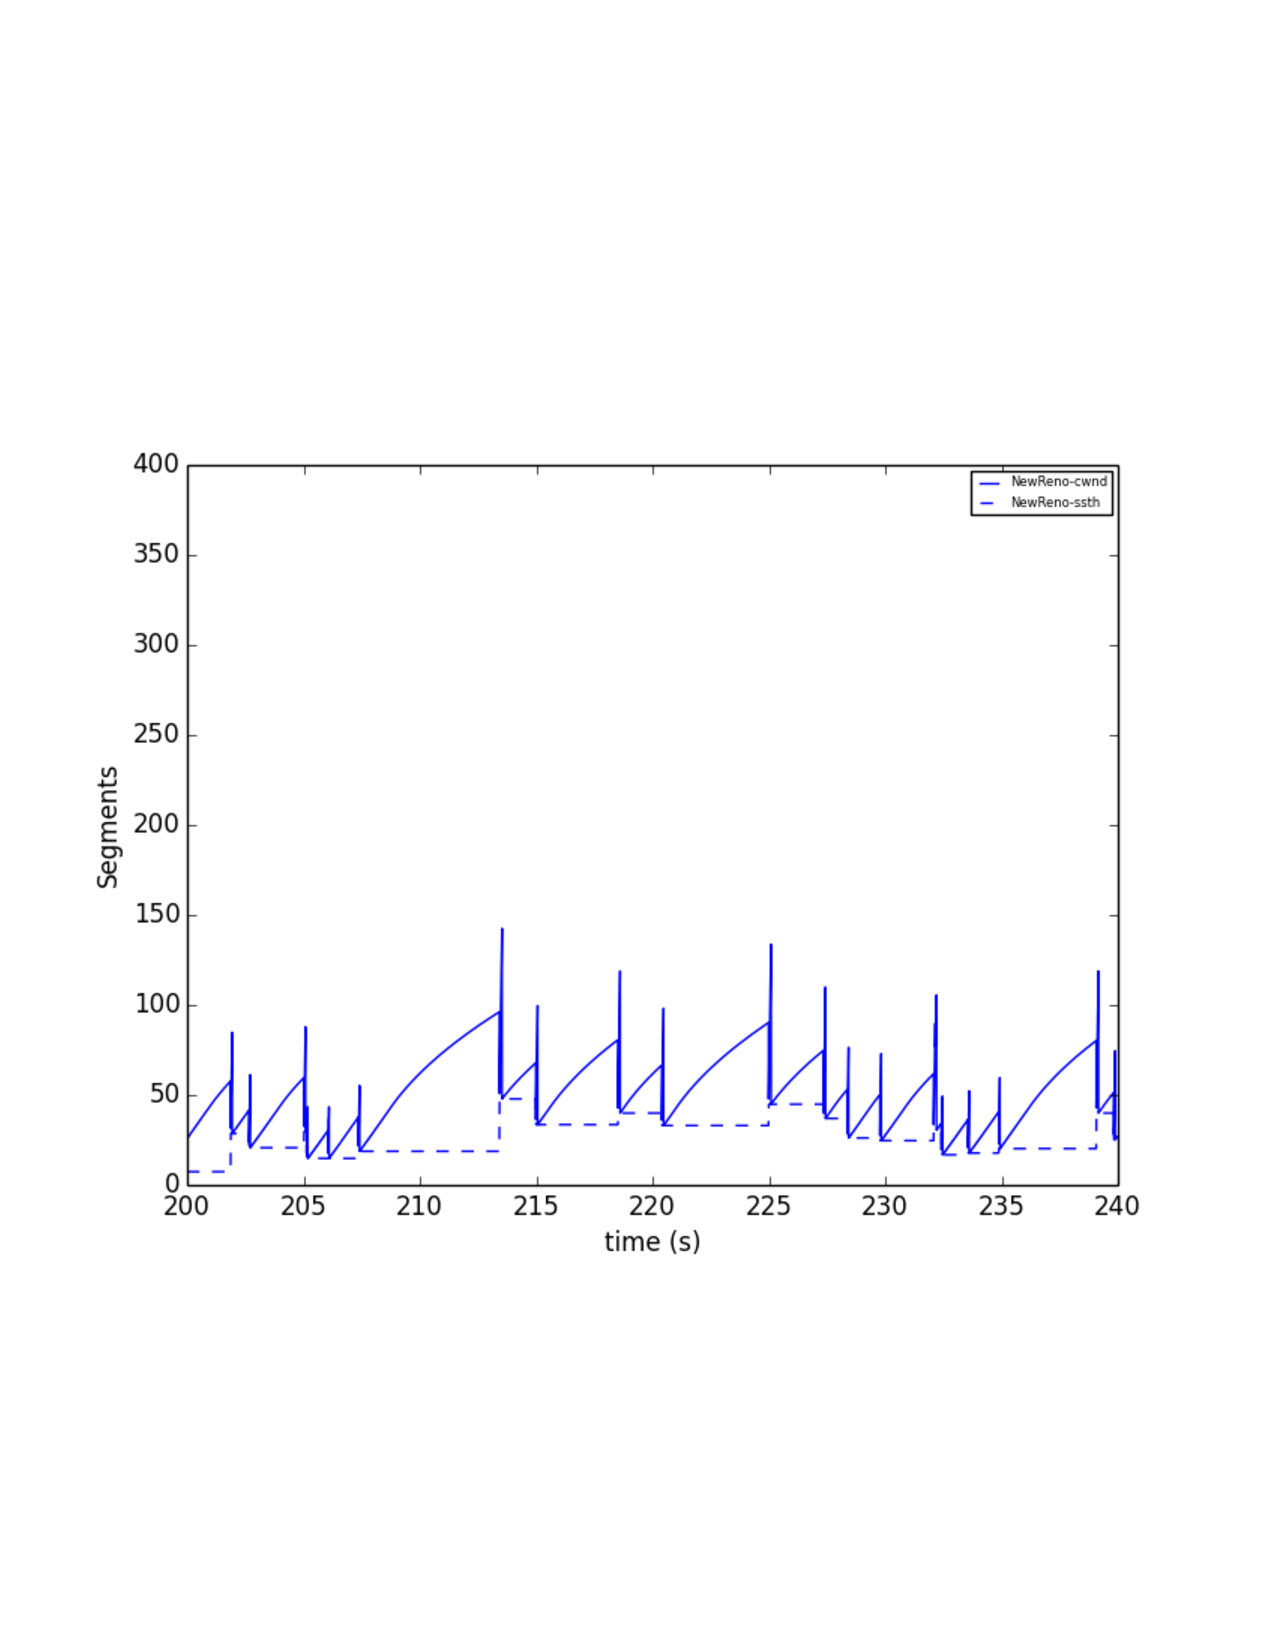
\includegraphics[trim=1cm 6.5cm 2.2cm 7.6cm, clip=true, scale=0.23]{inigo_test_results/repeatValidationPaper/finalVersion/PROD/PROD1.pdf}\label{a}} %3.24
\subfigure{ 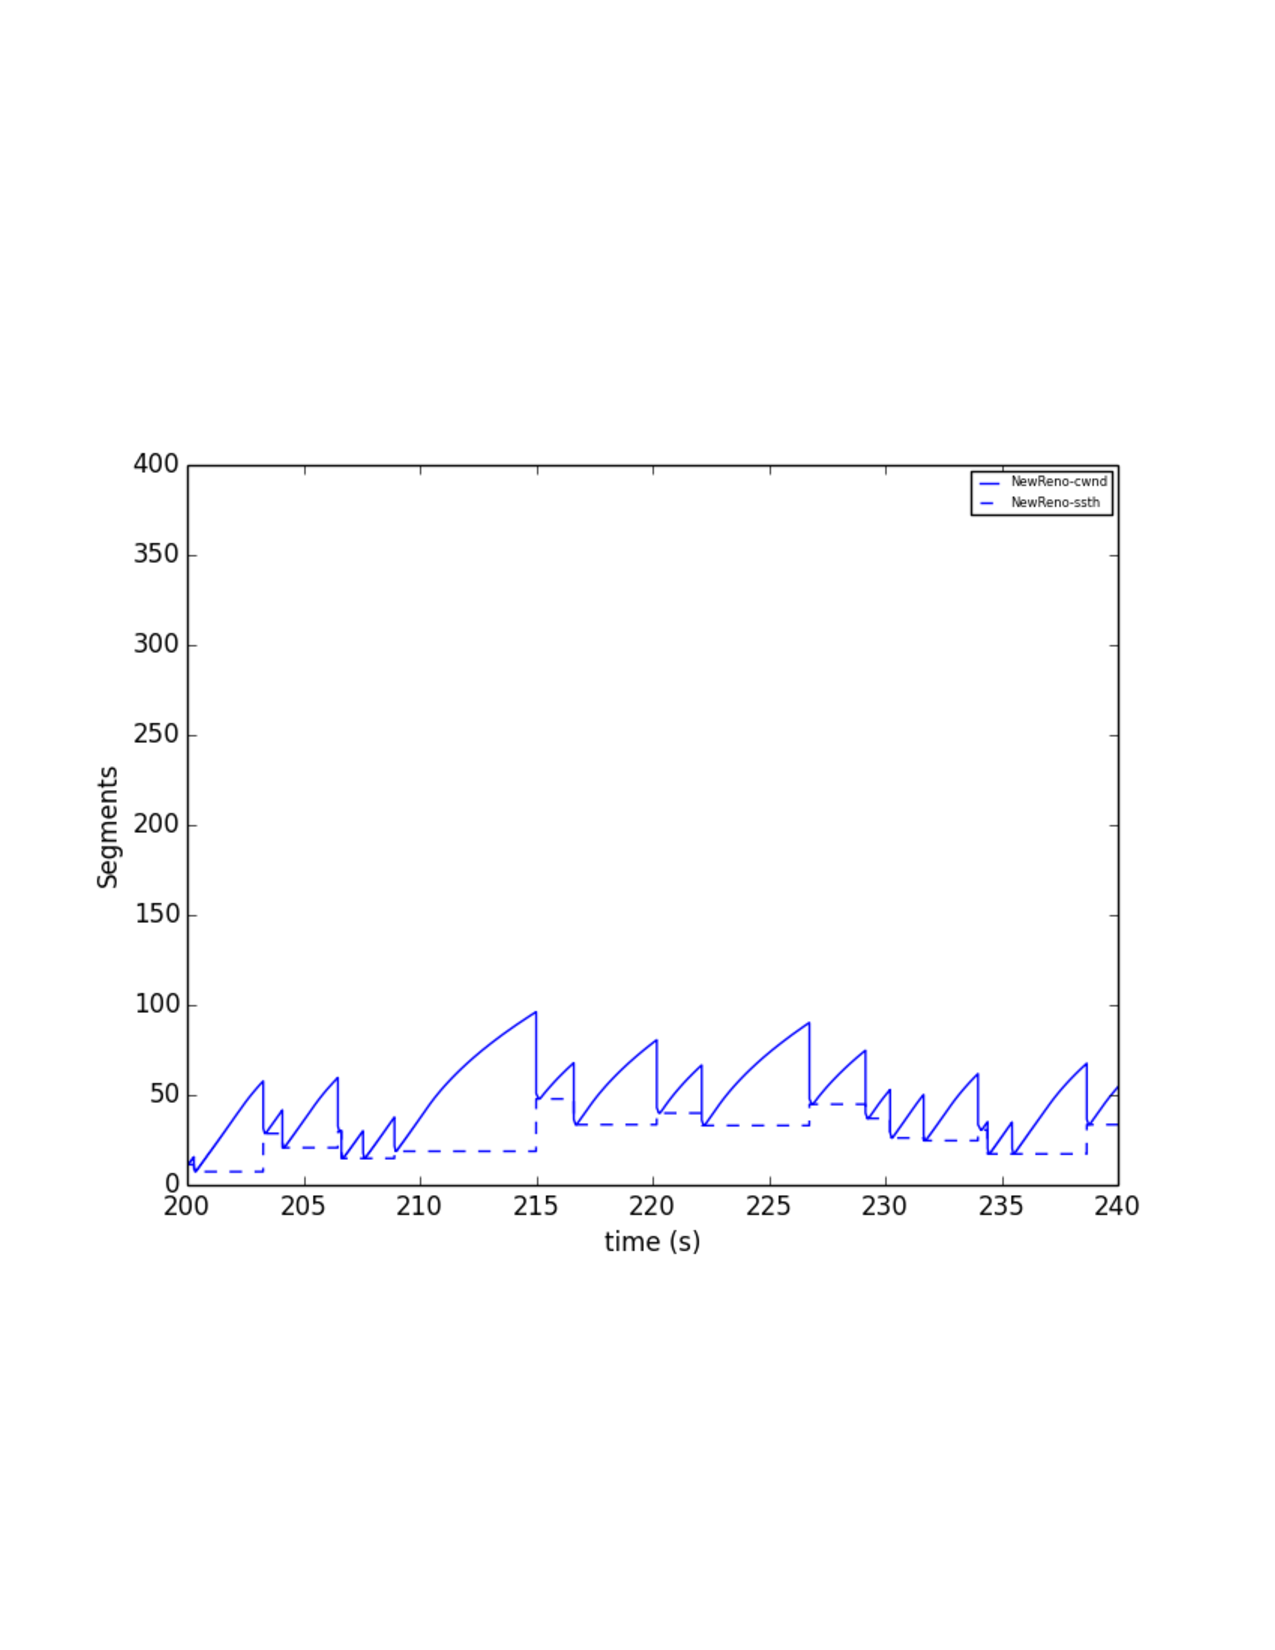
\includegraphics[trim=1cm 6.5cm 2.2cm 7.6cm, clip=true, scale=0.23]{inigo_test_results/repeatValidationPaper/finalVersion/PROD/PROD2.pdf}\label{b}} %3.24
\subfigure{ 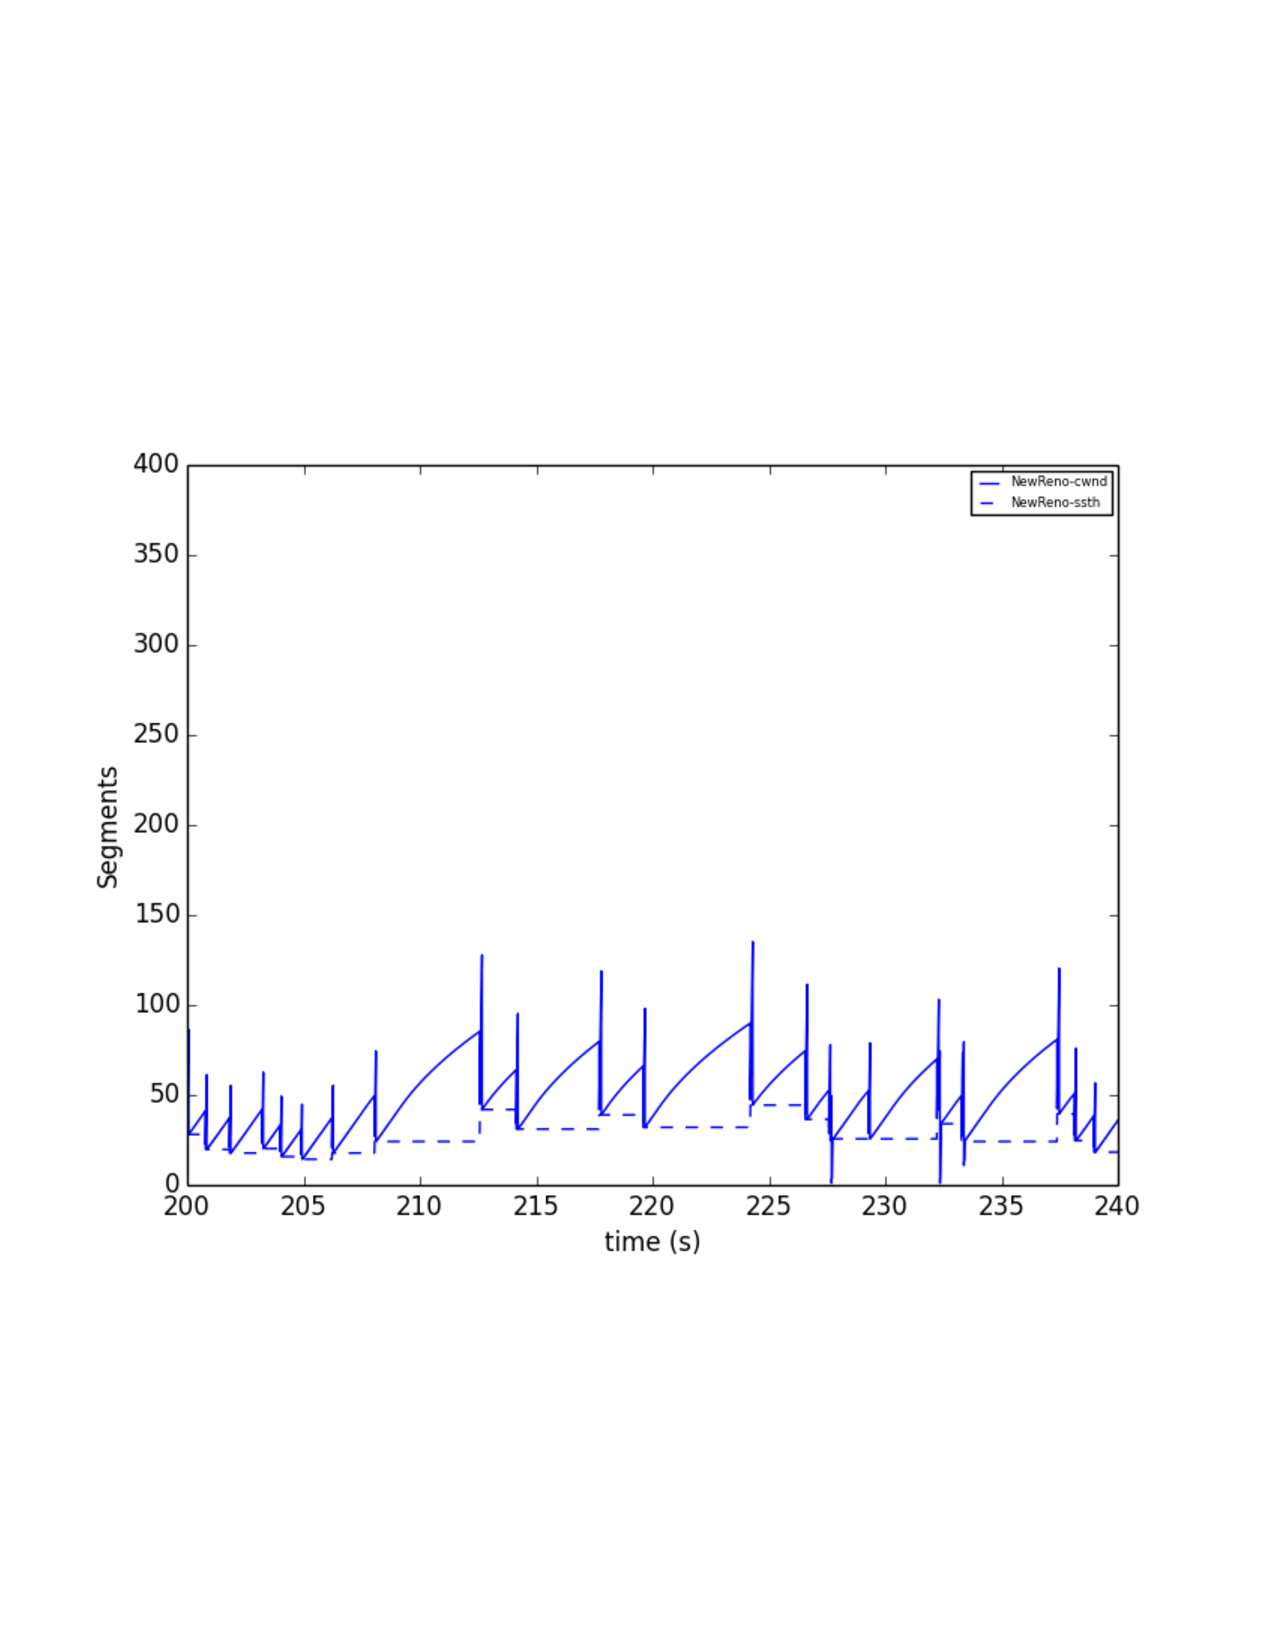
\includegraphics[trim=1cm 6.5cm 2.2cm 7.6cm, clip=true, scale=0.23]{inigo_test_results/repeatValidationPaper/finalVersion/PROD25/PROD25one.pdf}\label{c}} %3.25
\subfigure{ 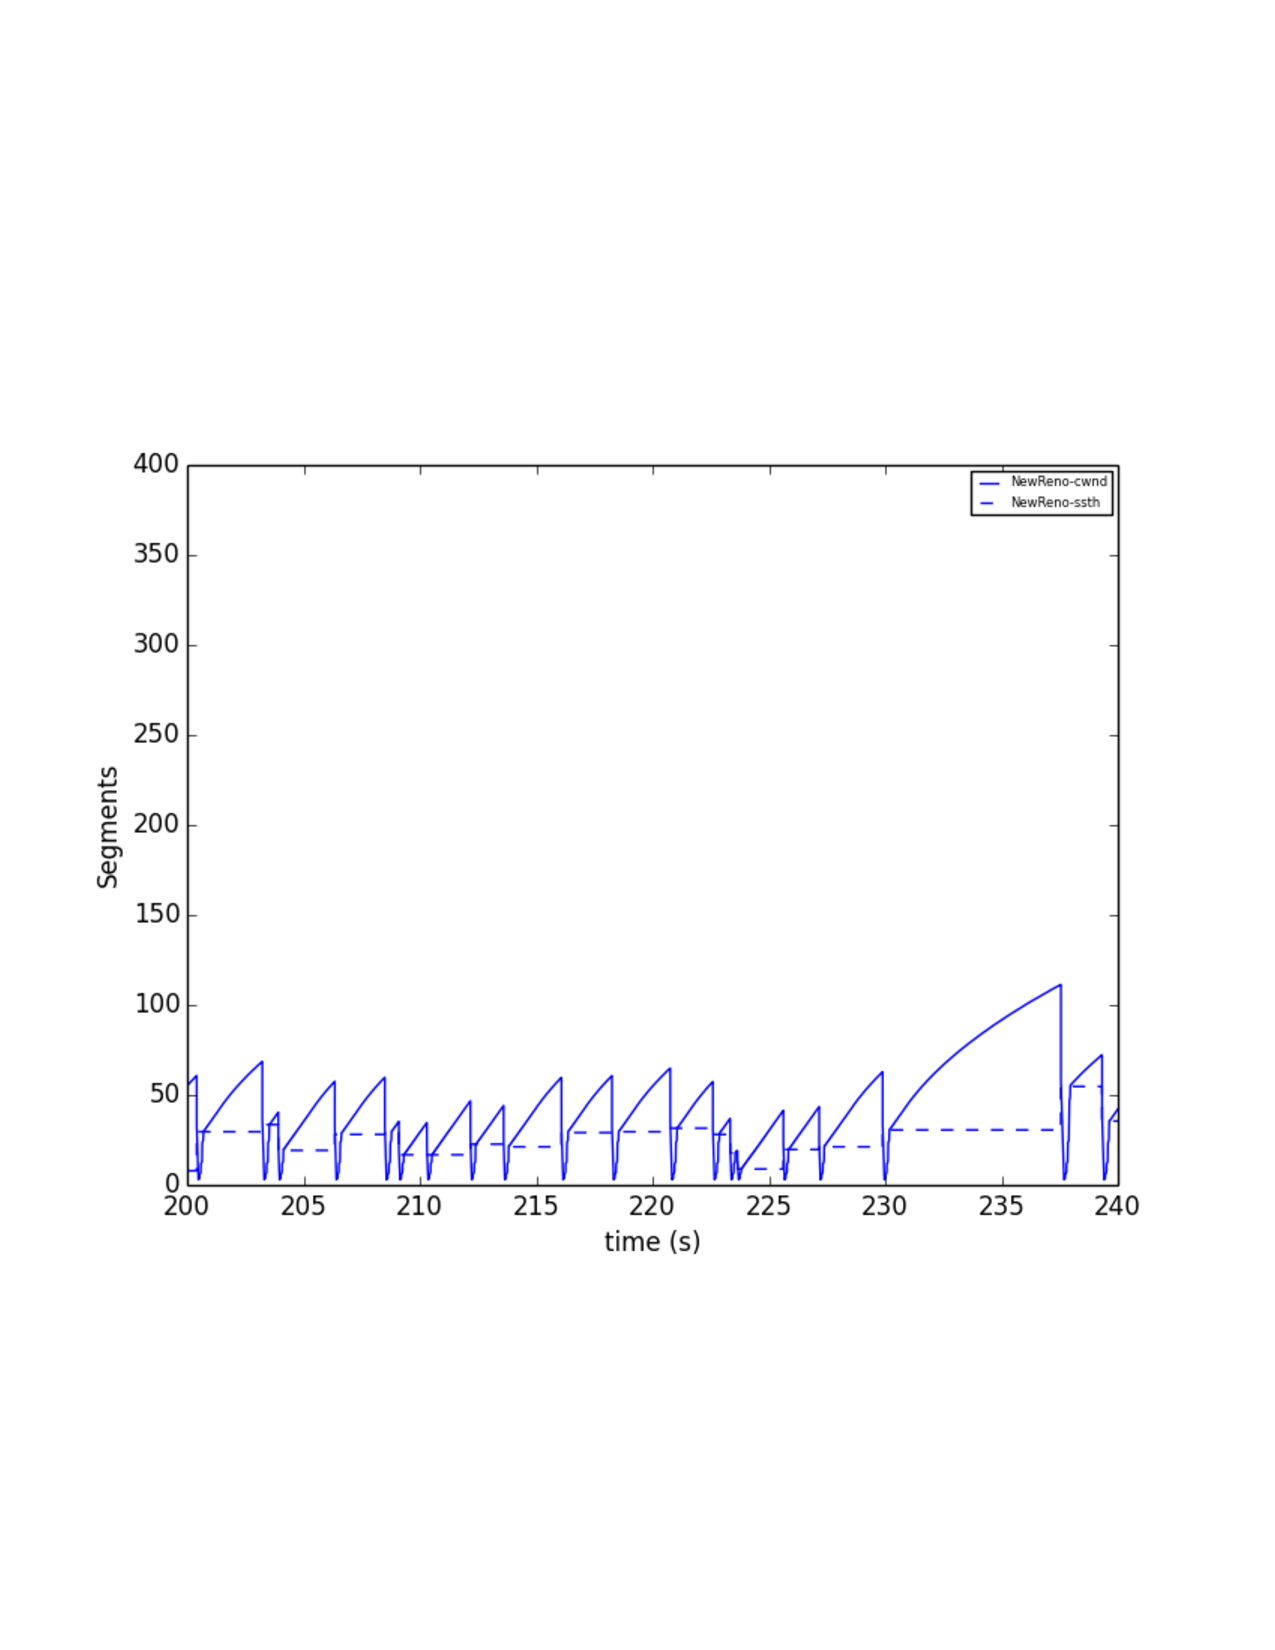
\includegraphics[trim=1cm 6.5cm 2.2cm 7.6cm, clip=true, scale=0.23]{inigo_test_results/repeatValidationPaper/finalVersion/PROD25/PROD25two.pdf}\label{d}} %3.25
\end{center}
\caption{40 seconds of a 600 second trace show congestion window and slow start threshold for NewReno in ns3-3.24 (top row) and ns3-3.25 (bottom row), with fast recovery on (left column) and off (right column).}
\label{fig:NS3Val}
\end{figure}

The parameters of the previous experiment included a packet loss rate of $10^{-3}$. Figure~\ref{fig:NS2Good} compares another experiment between NS3 versions 3.24 and 3.25, this time for experiments with a packet loss rate of 0. The two rows show two experiments with the left column providing results for version 3.24 and the right column providing results for version 3.25. The top row attempts to duplicate an experiment fist presented in Grieco et al\cite{NS2WP} and seen also in Abdeljaouad et al\cite{NS2Val}. This experiment originally included one forward flow with 10 back flows turning on and off but, due to the results discovered in attempting duplication, the experiment is presented here without the backflows. %finish writing this

\begin{figure}[h!]
\begin{center}
\subfigure{ 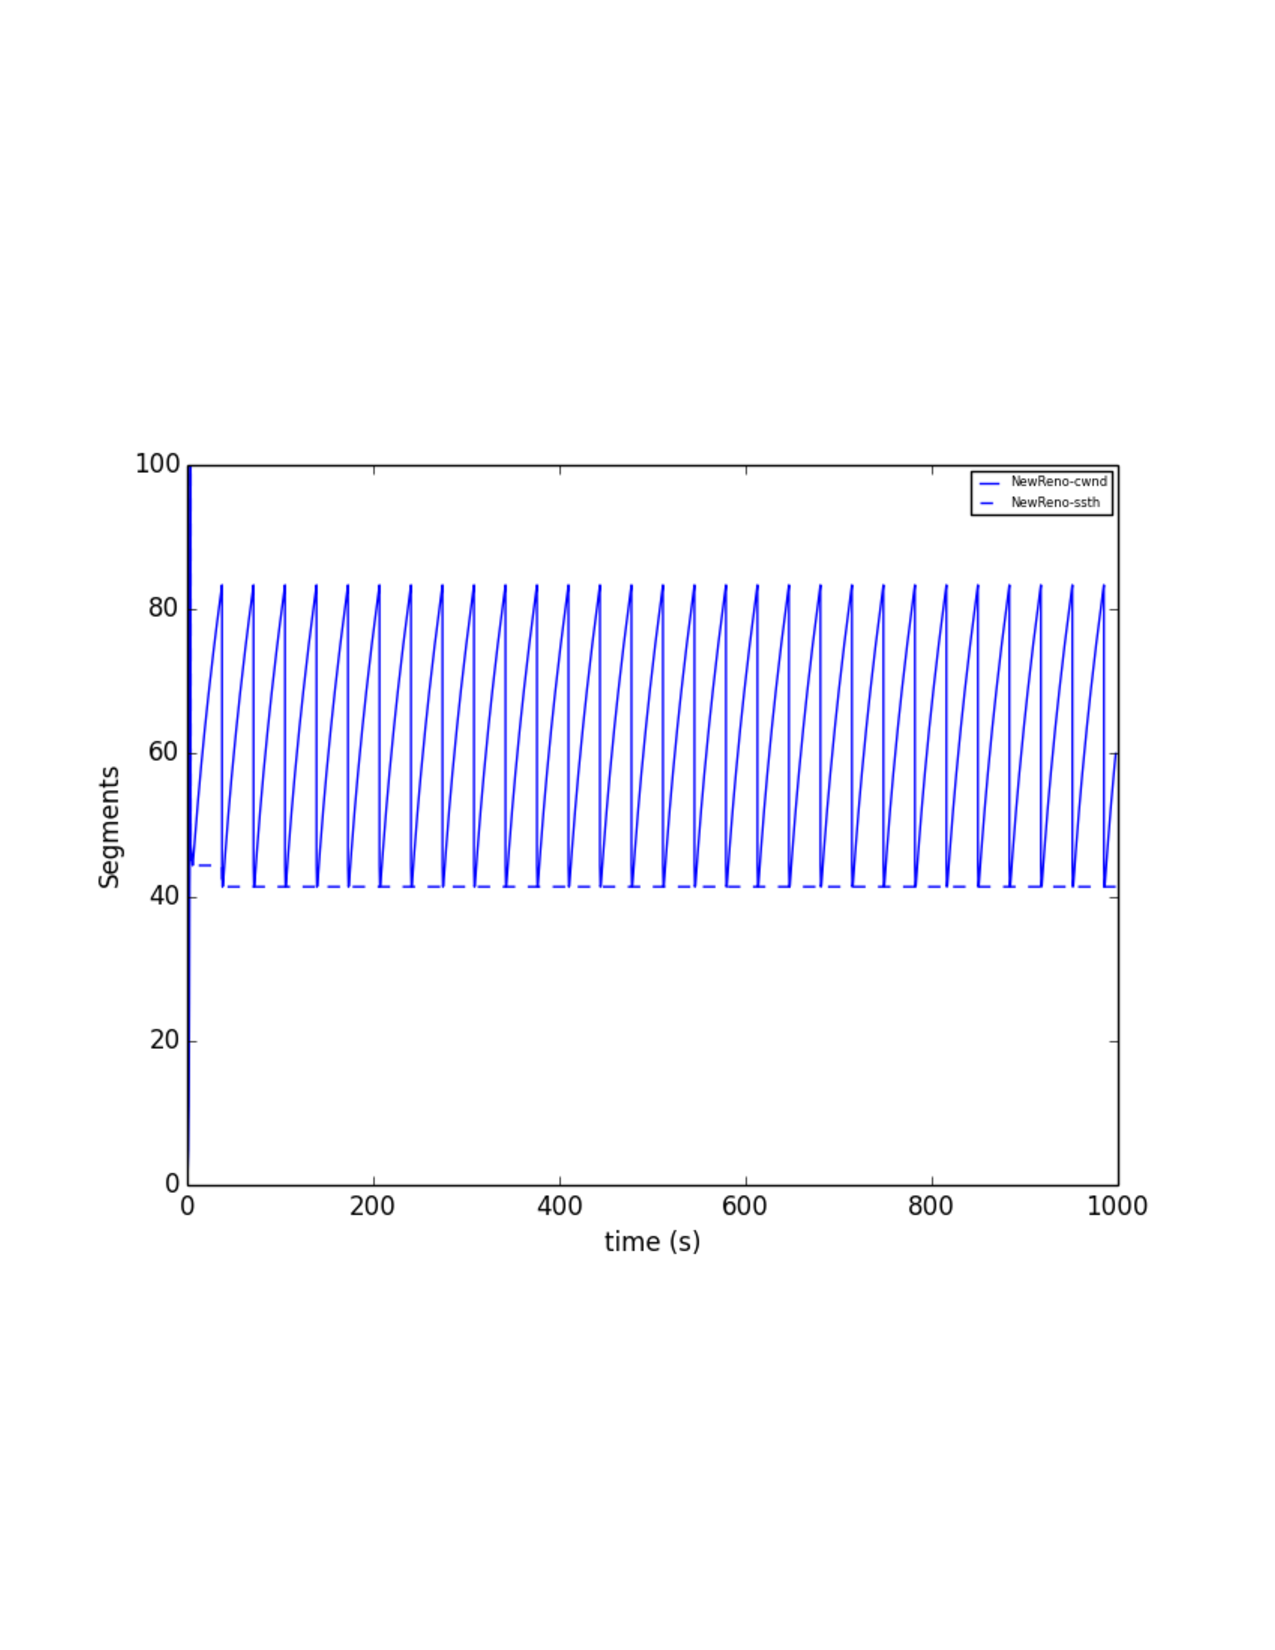
\includegraphics[trim=1cm 6.5cm 2.2cm 7.6cm, clip=true, scale=0.23]{inigo_test_results/repeatGoodpaper/24NewRenoG2.pdf}\label{a}} %3.24
\subfigure{ 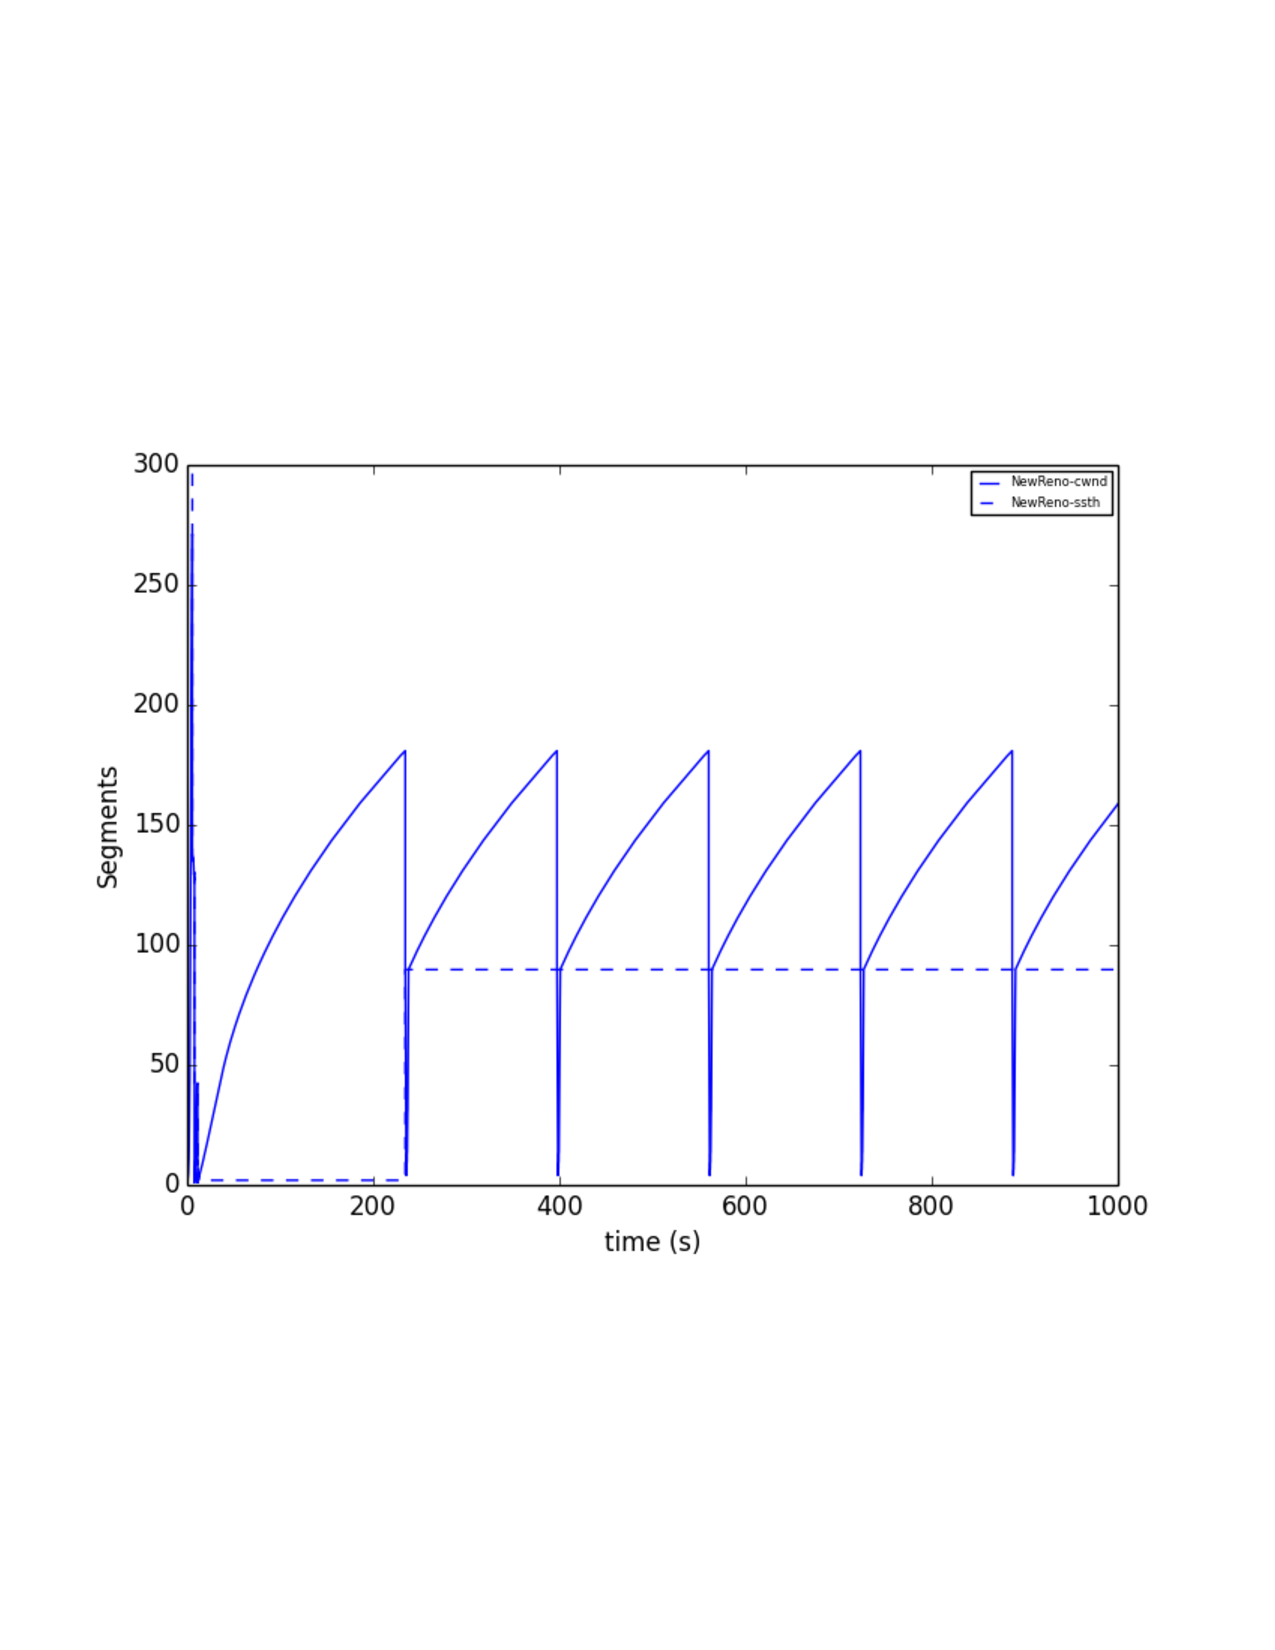
\includegraphics[trim=1cm 6.5cm 2.2cm 7.6cm, clip=true, scale=0.23]{inigo_test_results/repeatGoodpaper/GoodBetter.pdf}\label{b}} %3.25
\subfigure{ 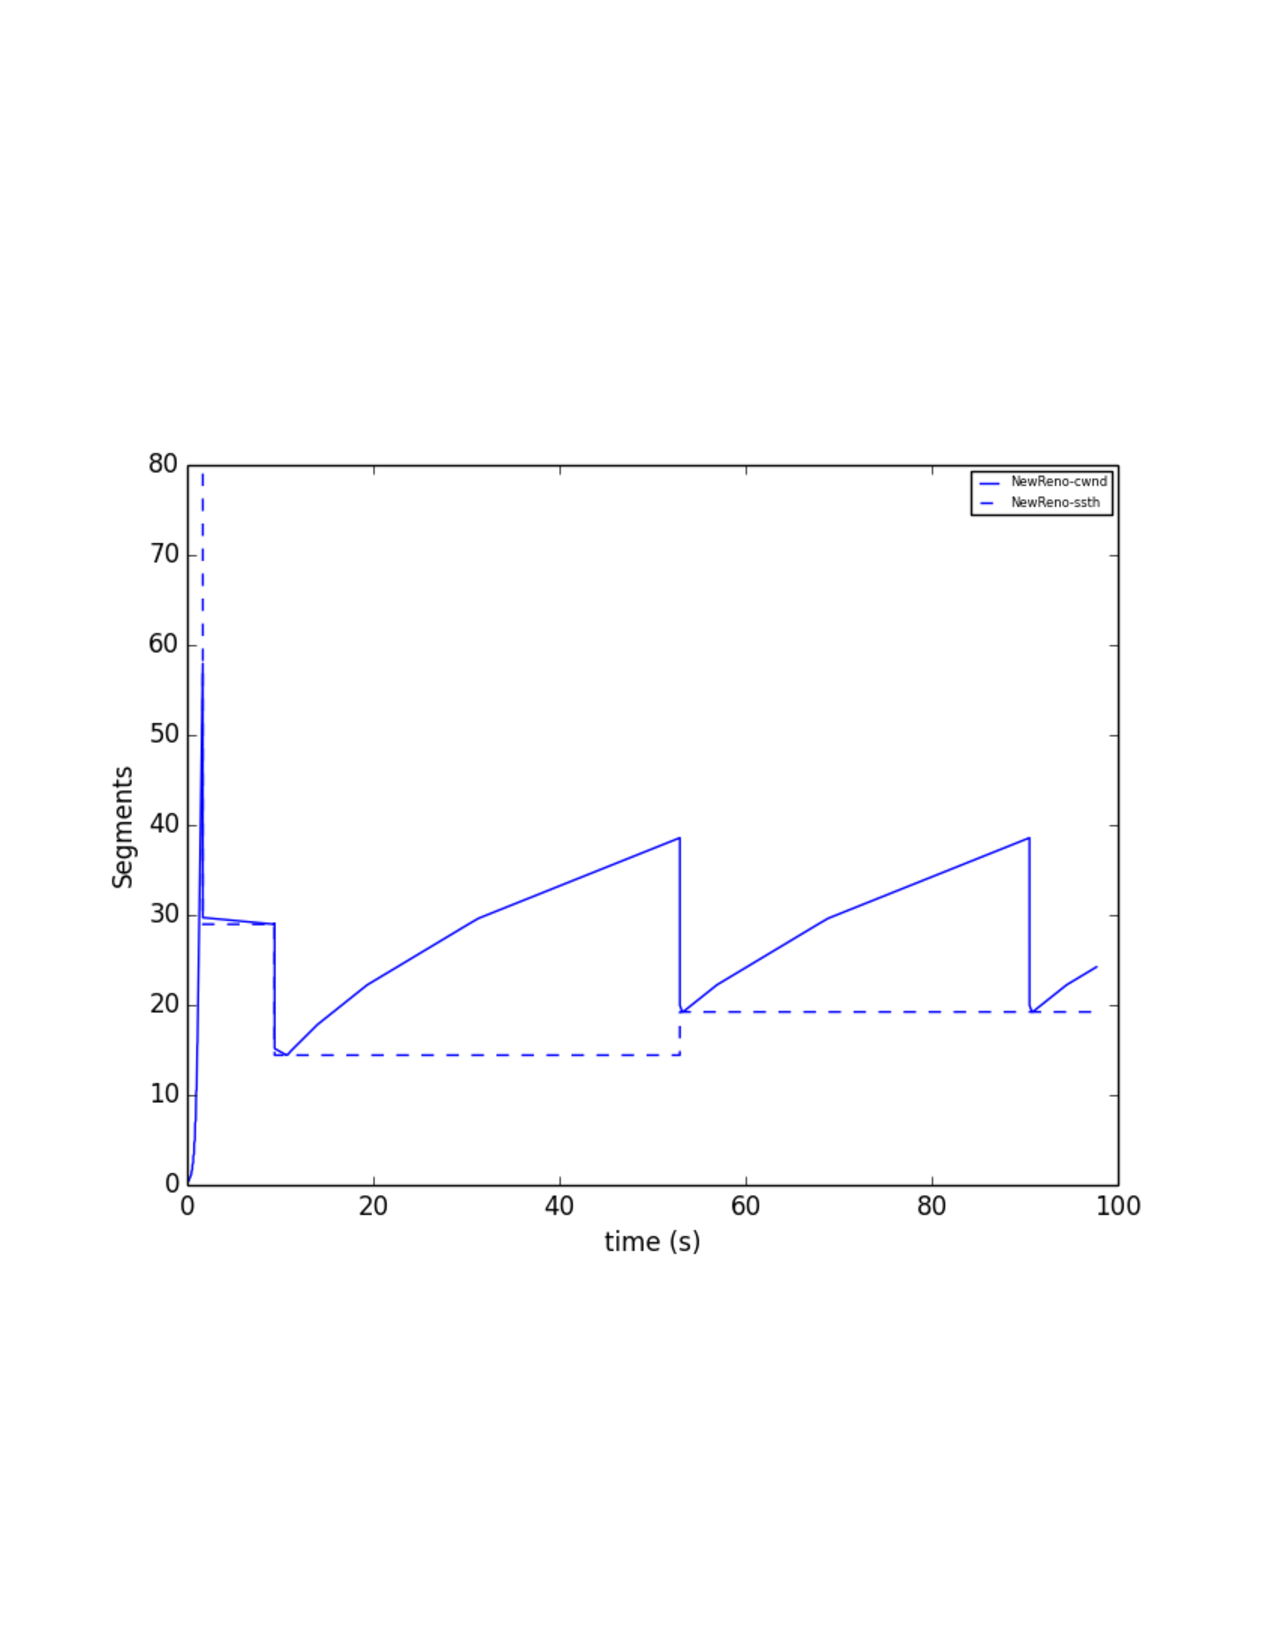
\includegraphics[trim=1cm 6.5cm 2.2cm 7.6cm, clip=true, scale=0.23]{inigo_test_results/repeatGoodpaper/provided242.pdf}\label{c}} %3.24
\subfigure{ 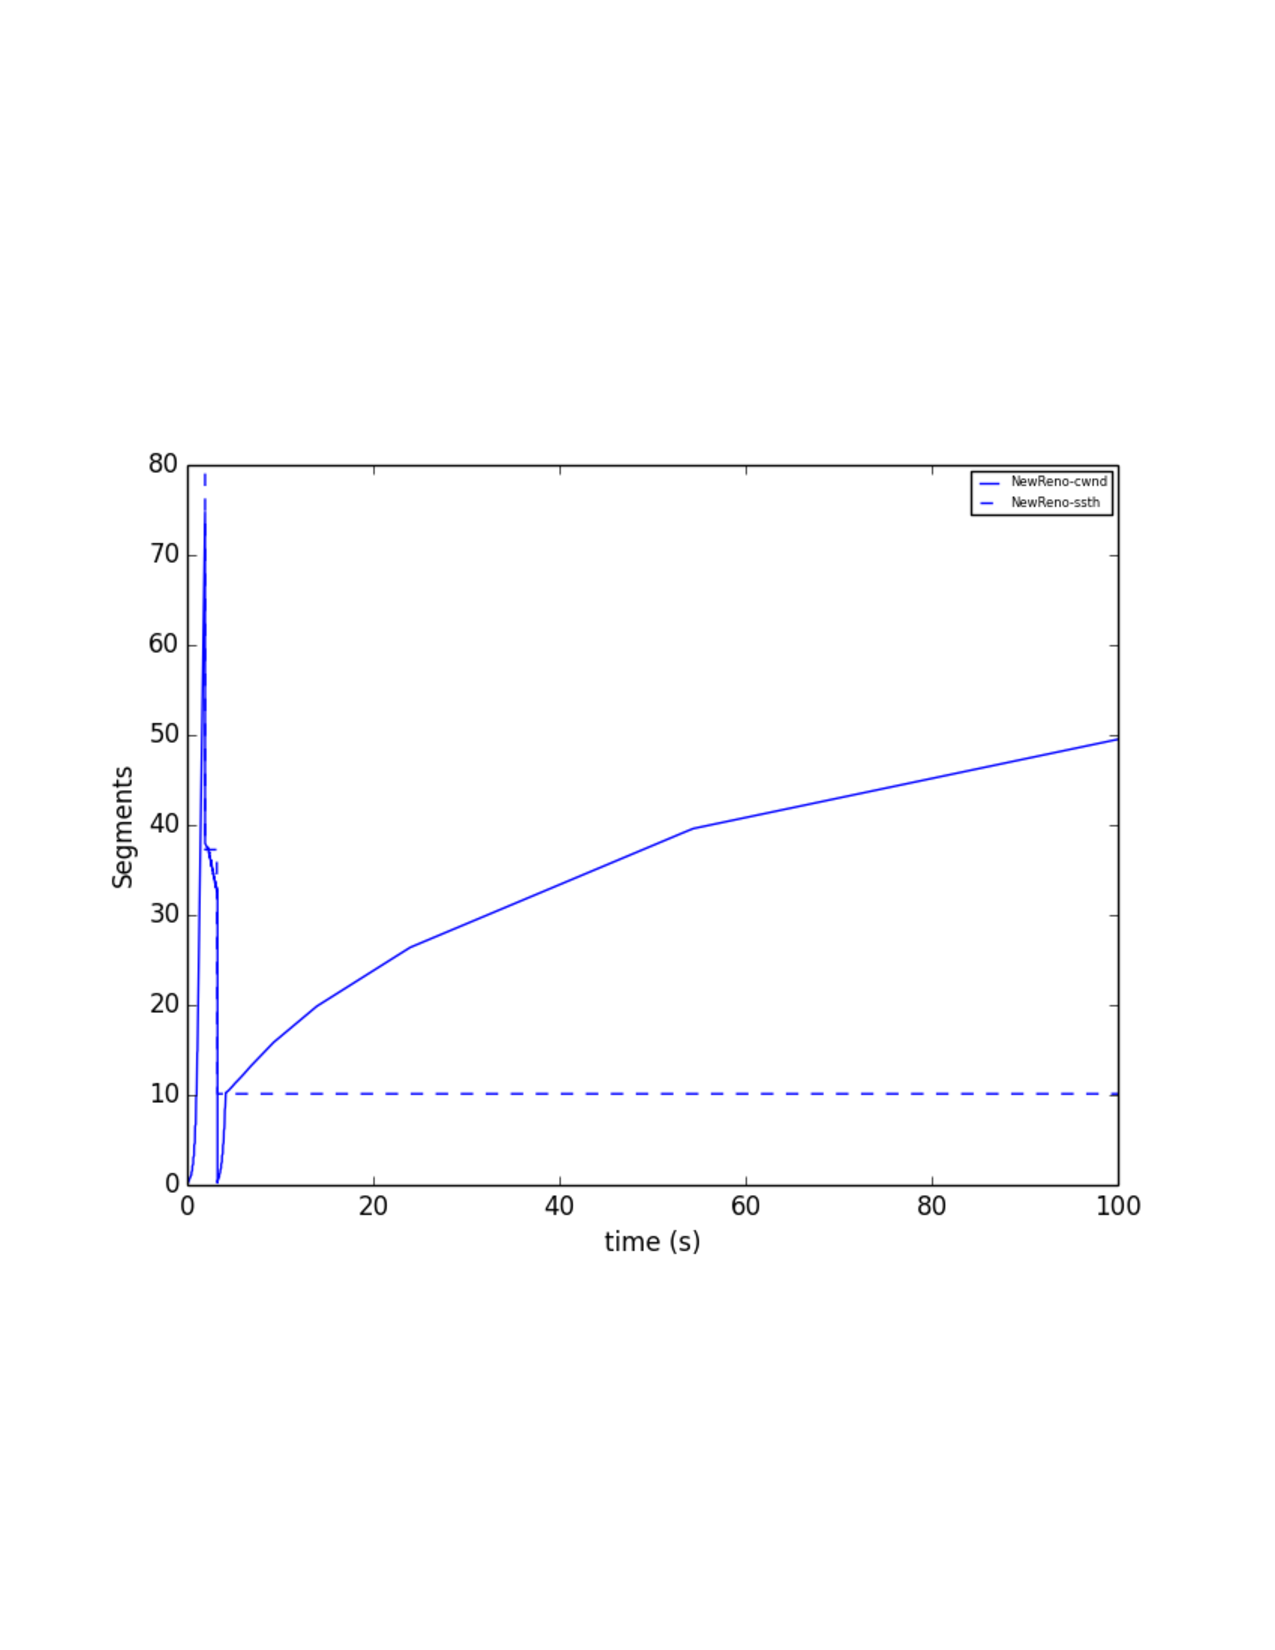
\includegraphics[trim=1cm 6.5cm 2.2cm 7.6cm, clip=true, scale=0.23]{inigo_test_results/repeatGoodpaper/provided25.pdf}\label{d}} %3.25
\end{center}
\caption{}
\label{fig:NS2Good}
\end{figure}

\cite{RFC6582}

\section{Discussion and Future Work} 

\section{Conclusion} 


\nocite{*}
\bibliographystyle{plain}
\bibliography{mybib}

%\appendix
%\chapter{Some Ancillary Stuff}

%Ancillary material should be put in appendices, which appear after the
%bibliography. 

\end{document}
